\chapter{方法论基础}
本文将首先从机器学习的角度介绍一些具有代表性的分类算法的运作步骤,并给出对应核心部分的MATLAB或R代码。然后将用小部分篇描述正则化,
交叉验证等关于模型选择和模型评价方面的知识。


\section{分类算法}

在机器学习与统计中,分类是指识别出样本所属类别的问题。分类问题在机器学习中属于有监督学习的范畴,即通过一组包含自变量与因变量(有限种取值)的训练模型,并通过模型对
其他没有因变量的样本进行预测。实务中的例子有垃圾邮件分类(通过邮件内的词语集合判断邮件是否为垃圾邮件),信用风险评级等。

现有的分类算法分为广义线性分类算法,支持向量机算法,决策树算法,神经网络算法几大类。下面对几种具体算法进行介绍。

\subsection{感知机}

感知机算法是由\textbf{Rosenblatt}于1957年所发明的一种二类分类的线性模型,可以看作最简单的前向神经网络。
在神经科学中,神经细胞的状态取决于从其它的神经细胞收到的输入信号量,及突触的强度(抑制或加强)。当信号量总和超过了某个阈值时,细胞体就会激动,产生电脉冲。
\textbf{Rosenblatt}被生物神经细胞的运作方式所启发,提出权重,阈值,激活函数等概念。
感知机的模型如下:


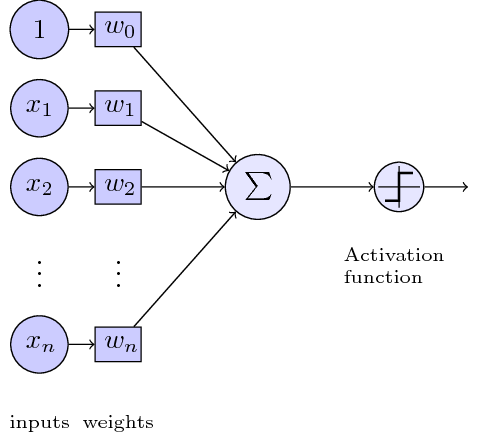
\includegraphics[scale = 0.4]{perceptron}




\subsection{Logistic回归}



\subsubsection{logit函数的背景,形态及特性}

logit函数的数学表达式为:

$f(x) = \frac{1}{1+\mathrm{e}^{-x}}$

其所具有的数学特性为:

$\frac{\mathrm d}{\mathrm d x} f(x) = f(x) * (1-f(x))$



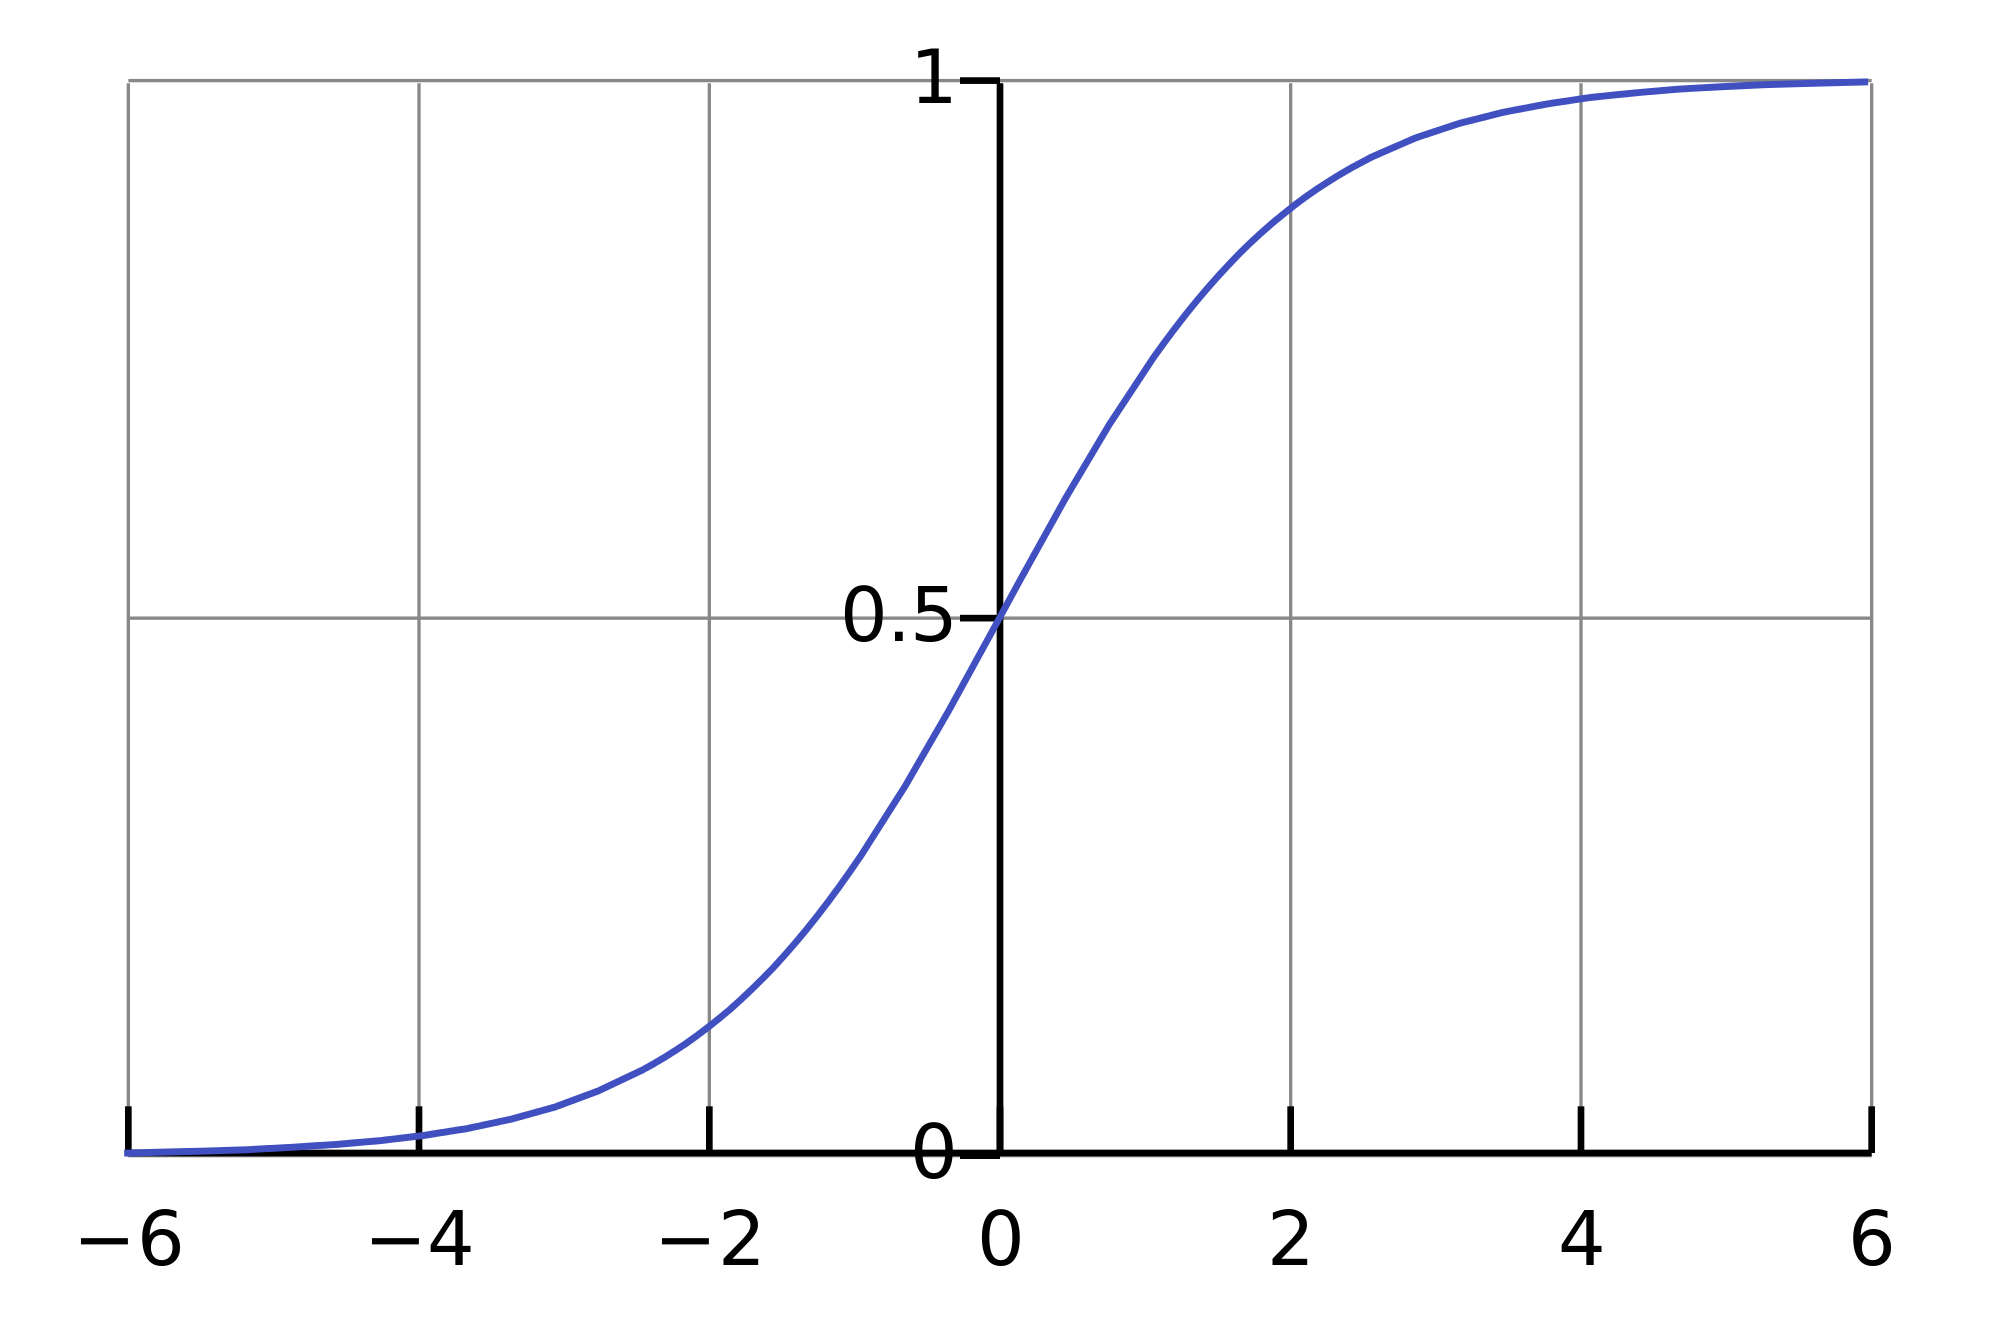
\includegraphics[scale = 0.1]{logistic}


logit函数的具有的生态学背景
https://www.zhihu.com/question/36714044

\begin{enumerate}
	\item 生物种群在无约束情况下,数量呈指数增长
	\item 增加约束,设立上限,则自然地得出有约束的公式
\end{enumerate}
此外,logit函数


\begin{minted}{python}
import numpy as np

def incmatrix(genl1,genl2):
m = len(genl1)
n = len(genl2)
M = None #to become the incidence matrix
VT = np.zeros((n*m,1), int)  #dummy variable

#compute the bitwise xor matrix
M1 = bitxormatrix(genl1)
M2 = np.triu(bitxormatrix(genl2),1) 

for i in range(m-1):
for j in range(i+1, m):
[r,c] = np.where(M2 == M1[i,j])
for k in range(len(r)):
VT[(i)*n + r[k]] = 1;
VT[(i)*n + c[k]] = 1;
VT[(j)*n + r[k]] = 1;
VT[(j)*n + c[k]] = 1;

if M is None:
M = np.copy(VT)
else:
M = np.concatenate((M, VT), 1)

VT = np.zeros((n*m,1), int)

return M
\end{minted}


\section{模型选择与验证}

我们首先借助一张图来说明欠拟合和过拟合,偏差和方差的概念。

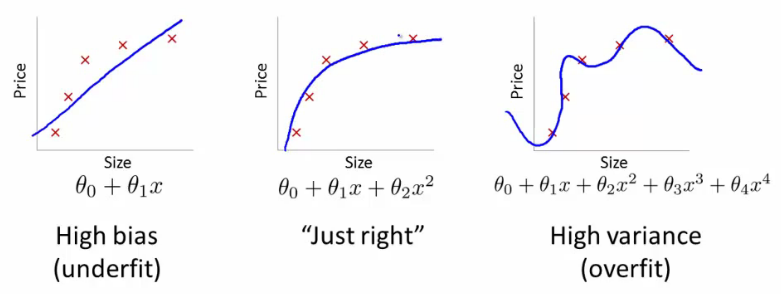
\includegraphics[scale = 0.8]{overfit}

我们可以看到,当用线性模型来拟合数据时造成了欠拟合,模型在训练集和测试集均有较大的误差。

而使用四次模型时,模型似乎完美地拟合了训练样本,但是由于模型过度追求拟合训练样本(将样本的误差,噪音等一并进行了学习),
破坏了其一般化(generalization)的能力,最终在测试集上也不会有较好的表现,这样的现象被称为过拟合。

下面用一个例子来进一步说明上面的问题并引入学习曲线的概念。

\begin{minted}{matlab}
%% =========== Part 1: Loading and Visualizing Data =============
X =  [-15.9368;-29.1530;36.1895;37.4922;-48.0588;-8.9415;15.3078;-34.7063;1.3892;-44.3838;7.0135;22.7627]

y = [2.1343;1.1733;34.3591;36.8380;2.8090;2.1211;14.7103;2.6142;3.7402;3.7317;7.6277;22.7524]

% m = Number of examples
m = size(X, 1);

% Plot training data
plot(X, y, 'rx', 'MarkerSize', 10, 'LineWidth', 1.5);

\end{minted}

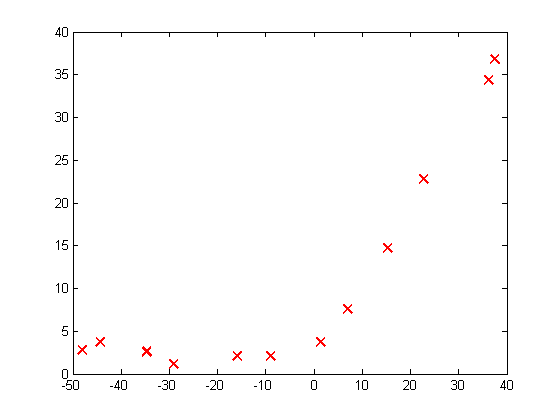
\includegraphics[scale = 1]{cv_scatter}

\begin{minted}{matlab}
%% =========== Part 2: Perform Linear Regression =============

%Add a column to X to compute theta0
X1 = [ones(m,1) X];

%Use Normal Equation to compute theta
theta = pinv((X1'*X1))*X1'*y;

%Plot the regression line
plot(X, y, 'rx', 'MarkerSize', 10, 'LineWidth', 1.5);
hold on;
plot(X, [ones(m, 1) X]*theta, '--', 'LineWidth', 2)
hold off;
\end{minted}

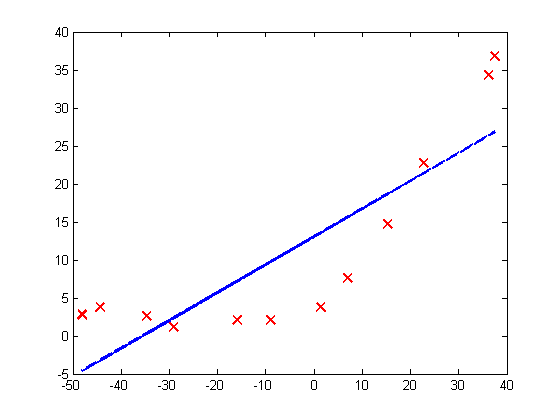
\includegraphics[scale = 1]{cv_linearReg}
